\title{Incentives in Casper the Friendly Finality Gadget}
\author{
        Vitalik Buterin \\
        Ethereum Foundation
}


\documentclass[12pt, final]{article}

% make in the latest NIPS format (as of this writing, 2017)

\usepackage[nonatbib,final]{nips_2017}
%\usepackage[nonatbib,final]{nips_2017}

\usepackage{color}
\usepackage{graphicx}
\DeclareGraphicsExtensions{.pdf,.eps,.png,.jpg}     % search for .pdf, then .eps, then .pngs, then .jpg

% look in these subdirectories for graphics referenced by \includegraphics
% each entry must end with a /
\graphicspath{{figs/}{figures/}{images/}{./}}

\newcommand*{\red}[1]{ \color{red} #1}

%\usepackage{tabularx}
\usepackage{url}
\usepackage{amsmath}

% this is for environments \subfigure and \subtable
\usepackage{subcaption}

% These packages are FORBIDDEN
%%%%%%%%%%%%%%%%%%%%%%%%%%%%%%%%%%%%%%%%%%%%%%%%%%%%%%%%
%\usepackage{lmodern} % messes up \textsc
%\usepackage{cite} % messes up NIPS
%\usepackage{fullpage} % messes up NIPS
%\usepackage{natbib} % messes up NIPS
%%%%%%%%%%%%%%%%%%%%%%%%%%%%%%%%%%%%%%%%%%%%%%%%%%%%%%%%

\usepackage{array}          % replacement for eqnarray.  Must be BEFORE \usepackage{arydshln}
\usepackage{units}          % for \nicefrac{\alpha}{\beta}


\usepackage{amsthm}     % for theorems
\newtheorem{definition}{Definition}

% text looks a little better
\usepackage{microtype}

\usepackage{wasysym}

\usepackage{textcomp, marvosym} % pretty symbols
\usepackage{booktabs}   % for much better looking tables

% for indicator functions
\usepackage{dsfont}

% For automatic capitalizaton of section names, etc.
\usepackage{titlesec,titlecaps}


\Addlcwords{is with of the and in}
\Addlcwords{of the}
\Addlcwords{and}
\titleformat{\section}[block]{}{\normalfont\Large\bfseries\thesection.\;}{0pt}{\formatsectiontitle}
\newcommand{\formatsectiontitle}[1]{\normalfont\Large\bfseries\titlecap{#1}}

\titleformat{\subsection}[block]{}{\normalfont\large\bfseries\thesubsection.\;}{0pt}{\formatsubsectiontitle}
\newcommand{\formatsubsectiontitle}[1]{\normalfont\large\bfseries\titlecap{#1}}





% for pretty Euler script
% \usepackage[mathscr]{euscript}
% \usepackage{bold-extra}





%\usepackage{subfig}
\usepackage{float} % for \subfloat

%%%%%%%%%%%%%%%%%%%%%%%%%%%%%%%%%%%%%%%%%%
%% More customizable Lists
%%%%%%%%%%%%%%%%%%%%%%%%%%%%%%%%%%%%%%%%%%
% Better symbols custom enumerative lists, define any symbol you'd like
% \usepackage{enumitem}


%%%%%%%%%%%%%%%%%%%%%%%%%%%%%%%%%%%%%%%%%%
%% Custom Symbols 
%%%%%%%%%%%%%%%%%%%%%%%%%%%%%%%%%%%%%%%%%%
% \xspace at the end of custom macros never screws up spacing.
\usepackage{xspace}



%%%%%%%%%%%%%%%%%%%%%%%%%%%%%%%%%%%%%%%%
%% Abbreviations you'll always want
%%%%%%%%%%%%%%%%%%%%%%%%%%%%%%%%%%%%%%%%
\newcommand*{\TODO}[1]{{\centering {\small \sffamily \color{red} #1} \vskip10pt }}
\newcommand*{\todo}[1]{{\small \sffamily [{\color{red} #1}]}}
\newcommand*{\q}[1]{{\small \sffamily [{\color{blue} #1}]}}
\newcommand*{\fix}[1]{{\sffamily [{\textnormal{\color{red} #1}}]}}



%-----------------------------------------------------------------------------
%  Cross references
%-----------------------------------------------------------------------------
% The following code defines how you make references to figures, tables, etc...
% It is defined in one place only, and can be modified for all references
% in the document at the same time.
% Instead of typing each time: "see Fig. \ref{myfig}" you can create a command
% \figref which will do the job. Then in text you only type \figref{myfig} and LaTeX
% will do the rest.
\newcommand{\tblref}[1]{Table~\ref{#1}}
%\renewcommand*{\figref}[1]{Fig.~\ref{#1}}
\renewcommand{\eqref}[1]{eq.~(\ref{#1})}
\newcommand{\Subref}[1]{(\subref{#1})}


\newcommand{\figref}[1]{Figure~\ref{#1}}
\newcommand{\Figref}[1]{Figure~\ref{#1}}
\newtheorem{theorem}{Theorem}
\newtheorem{lemma}[theorem]{Lemma}

%%%%%%%%%%%%%%%%%%%%%%%%%%%%%%%%%%%%%%%%

% for \sout{} for strikeout
% \usepackage[normalem]{ulem}


% for better manipulation of tables
\usepackage{makecell}
\renewcommand\theadfont{\bfseries}


%-----------------------------------------------------------------------------
%  Misc symbols that I like
%-----------------------------------------------------------------------------
\newcommand*{\opname}[1]{\operatorname{#1}}


\renewcommand*{\to}{\rightarrow}


%%%%




%% Special symbols we'll probably iterate on
%%%%%%%%%%%%%%%%%%%%%%%%%%%%%%%%%%%%%%%%%%%%%%%%%%%%%%
%\newcommand{\epoch}{ \mathscr{E} }
%\newcommand{\hash}{\ensuremath{ \mathscr{H} }}
%\newcommand{\epoch}{ {\footnotesize \textnormal{\textestimated} } }

\newcommand{\epoch}{\ensuremath{e}\xspace}
\newcommand{\hash}{\textnormal{h}\xspace}

%\newcommand{\epoch}{ \ensuremath{ \mathcal{E} } }
%\newcommand{\hash}{\ensuremath{ \mathcal{H} }}

%\newcommand{\epoch}{ \ensuremath{ \mathds{E} } }
%\newcommand{\hash}{\ensuremath{ \mathds{H} }}


\newcommand{\hashsource}{\ensuremath{\hash_{\star}}\xspace}
\newcommand{\epochsource}{\ensuremath{\epoch_{\star}}\xspace}

\newcommand{\signature}{\ensuremath{\mathcal{S}}\xspace}

\newcommand{\BIR}{\textsc{BIR}\xspace}
\newcommand{\BP}{\textsc{BP}\xspace}
\newcommand{\NCP}{\textsc{NCP}\xspace}
\newcommand{\NCCP}{\textsc{NCCP}\xspace}
\newcommand{\NPP}{\textsc{NPP}\xspace}
\newcommand{\NPCP}{\textsc{NPCP}\xspace}

\newcommand{\totaldeposit}{\textnormal{TD}\xspace}

\newcommand{\gamesymbol}{ \reflectbox{G} }

\newcommand{\msgPREPARE}{\textbf{\textsc{prepare}}\xspace}
\newcommand{\msgCOMMIT}{\textbf{\textsc{commit}}\xspace}

\newcommand{\epochLJ}{\ensuremath{\epoch_{\textnormal{LJ}}}\xspace}
\newcommand{\hashLJ}{\ensuremath{\hash_{\textnormal{LJ}}}\xspace} % we may not need this one


\newcommand{\epochLF}{\ensuremath{\epoch_{\textnormal{LF}}}\xspace}
\newcommand{\hashLF}{\ensuremath{\hash_{\textnormal{LF}}}\xspace} % we may not need this one

\newcommand{\GF}[1]{\mathds{GF}\left( #1 \right)\xspace}


%%%%%%%%%%%%%%%%%%%%%%%%%%%%%%%%%%%%%%%%%%%%%%%%%%%%%%

\begin{document}
\maketitle

\begin{center} \vspace{-15pt} {\red{\today}} \end{center}


\begin{abstract}
We give an introduction to the incentives in the Casper the Friendly Finality Gadget protocol, and show how the protocol behaves under individual choice analysis, collective choice analysis and griefing factor analysis. We define a ``protocol utility function'' that represents the protocol's view of how well it is being executed, and show the connection between the incentive structure that we present and the utility function. We show that (i) the protocol is a Nash equilibrium assuming any individual validator's deposit makes up less than $\frac{1}{3}$ of the total, (ii) in a collective choice model, where all validators are controlled by one actor, harming protocol utility hurts the cartel's revenue, and there is an upper bound on the ratio between the reduction in protocol utility from an attack and the cost to the attacker, and (iii) the griefing factor can be bounded above by $1$, though we will prefer an alternative model that bounds the griefing factor at $2$ in exchange for other benefits.
\end{abstract}


\section{Introduction}
\label{sect:intro}
\todo{Probably do a little more filler here citing previous PoS literature.}
Some of the prior Proof-of-Stake systems are \cite{bentov2016pos,king2012ppcoin,vasin2014blackcoin}.


\todo{define blocks, epochs}
A epoch is defined as a period of 100 blocks.  Epoch $k$ begins at block $k*100$ and ends at block $k*100 + 99$.  A \emph{checkpoint} for epoch $k$ is a block with number $k*100 - 1$.  In a perfect execution there will be exactly one checkpoint per epoch.  Due to to network latency or deliberate attacks there may be multiple competing checkpoints.  

\section{The Casper Protocol}
\label{sect:casperprotocol}
In the Casper protocol, there is a set of validators, and in each epoch validators have the ability to send two kinds of messages:


\begin{table}[h!bt]
	\centering
   
	\subfloat[\msgPREPARE format]{ \begin{tabular}{l l} \toprule
	\textbf{Notation} & \textbf{Description} \\
	\midrule
	\hash & the hash to justify \\
	\epoch & the current epoch \\
	$\hashsource$ & the most recent justified hash \\
	$\epochsource$ & the epoch containing hash $\hashsource$  \\
	\signature & signature from the validator's private key of the tuplet $(\hash,\epoch,\hashsource,\epochsource)$. \\
	\bottomrule
	\end{tabular} \label{tbl:prepare} }
	
	\subfloat[\msgCOMMIT format]{ \begin{tabular}{l l} \toprule
	\textbf{Notation} & \textbf{Description} \\
	\midrule
	\hash & the hash to finalize \\
	\epoch & the current epoch \\
	\signature & signature from the validator's private key \\
	\bottomrule
	\end{tabular} 
	\label{tbl:commit} }	
	\caption{The schematic of the \msgPREPARE and \msgCOMMIT messages.}
	\label{fig:messages}
\end{table}


Each validator has a \emph{deposit size}; when a validator joins their deposit size is equal to the number of coins that they deposited, and from there on each validator's deposit size rises and falls with rewards and penalties. For the rest of this paper, when we say ``$\nicefrac{2}{3}$ of validators'', we are referring to a \emph{deposit-weighted} fraction; that is, a set of validators whose sum deposit size equals to at least $\frac{2}{3}$ of the total deposit size of the entire set of validators. We also use ``$\nicefrac{2}{3}$ Prepares'' and ``$\nicefrac{2}{3}$ Commits'' as shorthand for ``$\frac{2}{3}$ of deposit-weighted validators sent Prepares/Commits''.

Every hash $\hash$ has one of three possible states: \emph{fresh}, \emph{justified}, and \emph{finalized}.  Every hash starts as \emph{fresh}.  The hash at the beginning of the current epoch converts from fresh to \emph{justified} if, during the current epoch $\epoch$, $\nicefrac{2}{3}$ Prepares are sent of the form 

\begin{equation}
\langle \msgPREPARE, \epoch, \hash, \epochsource, \hashsource, \signature \rangle 
\label{eq:msgPREPARE}
\end{equation}

for some specific $\epochsource$ and $\hashsource$.  A hash $\hash$ can only be justified if and only if its $\hashsource$ is already justified or finalized.

Additionally, a hash converts from justified to \emph{finalized}, if $\nicefrac{2}{3}$ Commits  

\begin{equation}
\langle \msgCOMMIT, \epoch, \hash, \signature \rangle \; ,
\label{eq:msgCOMMIT}
\end{equation}

for the same \epoch and \hash as in \eqref{eq:msgPREPARE}.  The $\hash$ is the block hash of the block at the start of the epoch.  A hash $\hash$ being justified entails that all fresh (non-finalized) ancestor blocks are also justified.  A hash $\hash$ being finalized entails that all ancestor blocks are also finalized, regardless of whether they were previously fresh or justified.  An ``ideal execution'' of the protocol is one where, at the start of every epoch, every validator Prepares and Commits the first blockhash of each epoch, specifying the same $\epochsource$ and $\hashsource$. We wish to incentivize this ideal execution.

Possible deviations from this ideal execution that we want to minimize or avoid include:

\begin{itemize}
\item Violating any of the two Casper Commandments. \cite{minslashing}  To violate either Commandment is to forfeit one's \emph{entire deposit}.

\begin{enumerate}
   \item[\textbf{I.}] \textsc{A validator shalt not publish two nonidentical Prepares with the same $\epoch$ value.}
   
   This is equivalent to that each validator may Prepare to exactly one (\hash, \epochsource, \hashsource) triplet per epoch.

    \item[\textbf{IIa.}] \textsc{A validator shalt not publish an Commit between a Prepare jump.} 
    
    Equivalently, a validator will not publish


%    \item[\textbf{II.}] \textbf{\textsc{prepare\_commit\_consistency}}. A validator shalt not publish an incompatible Prepare/Comment pairing.  Equivalently, ro4 a single hash $\hash$, a validator will not publish

\begin{equation*}
\langle \msgPREPARE, \epoch_p, \hash_p, \epochsource, \hashsource, \signature \rangle \hspace{0.5in} \textnormal{\textsc{and}} \hspace{0.5in} \langle \msgCOMMIT, \epoch_c, \hash_c, \signature \rangle \;, 
\label{eq:msgPREPARE}
\end{equation*}

where the epochs satisfy $\epochsource < \epoch_c < \epoch_p$.


    \item[\textbf{IIb.}] \textsc{A validator shall only publish compatible Prepare/Commit pairings.} 
    
    Equivalently, for a single hash $\hash$, a validator shall only publish


%    \item[\textbf{II.}] \textbf{\textsc{prepare\_commit\_consistency}}. A validator shalt not publish an incompatible Prepare/Comment pairing.  Equivalently, ro4 a single hash $\hash$, a validator will not publish

\begin{equation*}
\langle \msgPREPARE, \epoch_p, \hash, \epochsource, \hashsource, \signature \rangle \hspace{0.5in} \textnormal{\textsc{and}} \hspace{0.5in} \langle \msgCOMMIT, \epoch_c, \hash, \signature \rangle \;, 
\label{eq:msgPREPARE}
\end{equation*}

where the epochs satisfy $\epochsource < \epoch_p \leq \epoch_c$.



%    \item \textbf{\textsc{prepare\_req}}. A validator shalt not Prepare with a $\hashsource$ that is not \emph{justified}.

%    \item \textbf{\textsc{commit\_req}}. If a validator Commits an unjustified hash, the validator is penalized.
%\item[\textbf{III.}] \todo{Don't we need another saying don't Commit on an unjustified hash?}
     \end{enumerate}


%\item During some epoch, we do not get $\nicefrac{2}{3}$ Prepares for the same $(h, \hashsource, \epochsource)$ combination.
%\item During some epoch, we do not get $\nicefrac{2}{3}$ Commits for the $hash$ that received $\nicefrac{2}{3}$ prepares. \todo{there can be multiple hashes that received 2/3 prepares, right?}

\item By the end of epoch \epoch, the first blockhash of epoch \epoch is not 100\% justified or is not 100\% finalized.
\end{itemize}

All Prepares with an $\hashsource$ that is not justified is ignored.
All Commits from unjustified hashes are ignored.

Each validator only see the blockchain's own history, including messages that were passed in. \todo{Are Commits/Prepares stored on-chain?}
%In a history that contains some blockhash $H$, our strategy is to reward validators who Prepared and Committed $H$, and not reward prepares or commits for any hash $H^\prime \ne H$.

The blockchain state stores the latest justified epoch and hash, $\epochLJ$ and $\hashLJ$, and only rewards Prepares whose $\epochsource = \epochLJ$ and $\hashsource = \hashLJ$. These two techniques will help to coordinate validators toward Preparing and Committing a single epoch \epoch and hash \hash.

Let $\totaldeposit$ be the current \emph{total amount of deposited coins}, and $\epoch - \epochLF$ be the number of epochs since the last finalized epoch.


\section{Rewards and Penalties}

We define the following nonnegative functions, all of which return a nonnegative scalar with no units.  Technically these values can exceed 1.0, but in practice they will be rarely exceed $0.01$: 

\begin{itemize}
\item $\BIR(\totaldeposit)$: returns the base interest rate paid to a validator, taking as an input the current total quantity of deposited coins.

\item $\BP(\totaldeposit, \epoch - \epochLF )$: returns the ``base penalty constant''---a value expressed as a percentage rate that is used as the scaling factor for all penalties; for example, if at the current time $\BP(\cdot, \cdot, \cdot) = 0.001$, then a penalty of $1.5$ means a validator loses $0.15\%$ of their deposit. Takes as inputs the current total quantity of deposited coins $\totaldeposit$, the current epoch $e$ and the last finalized epoch \epochLF. Note that in a perfect protocol execution, $\epoch - \epochLF = 1$.

\item $\NPCP(\alpha)$ (``non-prepare collective penalty''): if $\alpha$ of validators ($0 \leq \alpha \leq 1$) are not seen to have Prepared during an epoch, then \emph{all} validators are charged a penalty of $\NCCP(\alpha)$. $\NPCP$ must be monotonically increasing, and satisfy $\NPCP(0) = 0$.

\item $\NCCP(\alpha)$ (``non-commit collective penalty''): if $\alpha$ of validators ($0 \leq \alpha \leq 1$) are not seen to have Committed during an epoch, and that epoch had a justified hash so any validator \emph{could} have Committed, then all validators are charged a penalty proportional to $\NCCP(\alpha)$. $\NCCP$ must be monotonically increasing, and satisfy $\NCCP(0) = 0$.
\end{itemize}

We also define the following nonnegative constants:
\begin{itemize}
    \item $\NPP$ (``non-prepare penalty''): the penalty for not Preparing any block during the epoch. \todo{correct?}
    \item $\NCP$ (``non-commit penalty''): the penalty for not Committing any block during the epoch, if there was a justified hash which the validator \emph{could} have Committed. \todo{correct?}
\end{itemize}


Note that a validator publishing a Prepare/Commit doesn't entail escaping a \NPP/\NCP; it could be the case that either because of high network latency or a malicious majority censorship attack, the Prepares and Commits are not included into the blockchain in time and so the incentivization mechanism does not see them. Likewise, for $\NPCP$ and $\NCCP$, the $\alpha$ input is the proportion of validators whose Prepares and Commits are \emph{not visible}, not the proportion of validators who \emph{tried to send} a Prepare/Commit. 

When we talk about Preparing and Committing the ``correct value'', we are referring to the hash \hash and the parent epoch $\epochsource$ and parent hash $\hashsource$.

We define the following reward and penalty schedule.  This is the procedure for rewards and penalties, and is the entirety of the incentivization structure.  It runs at the \emph{end} of every epoch:
    \begin{enumerate}
    \item All validators get a reward of $\BIR(\totaldeposit)$ (e.g., if $\BIR(\totaldeposit) = 0.0002$ then a validator with $10,000$ coins deposited gets a per-epoch reward of $2$ coins)
    \item If the protocol does not see a Prepare from a given validator during the epoch, the validator is penalized $\BP(\totaldeposit, \epoch - \epochLF) * \NPP$ \todo{how does the incentive mechanism know \epoch?}
    \item If the protocol does not see a Commit from a given validator during the epoch, and a block was justified (so a Commit \emph{could have} been seen), the validator is penalized $\BP(\totaldeposit, \epoch - \epochLF) * \NCP$.
    \item If the protocol saw Prepares from proportion $p$ validators during the epoch, then \emph{every} validator is penalized $\BP(\totaldeposit, \epoch - \epochLF) * \NPCP(1 - p)$.
    \item If the protocol saw Commits from proportion $p$ validators during the epoch, and a block was justified (so validators \emph{could have} Commited), then \emph{every} validator is penalized $\BP(\totaldeposit, \epoch - \epochLF) * \NCCP(1 - p)$.
    \item The blockchain's recorded \epochLF and \hashLF are updated to the latest values. \todo{correct?}
    \end{enumerate}




\section{Three theorems}

We seek to prove the following:

\begin{theorem}[\todo{First theorem}]
\label{theorem1}
If no validator has more than $\frac{1}{3}$ of the total deposit, i.e., $\max_i(D) \leq \frac{\totaldeposit}{3}$, then Preparing the last blockhash of the previous epoch and then Committing that hash is a Nash equilibrium. (Section \ref{sect:indivchoice})
\end{theorem}

\begin{theorem}[\todo{Second theorem}]
\label{theorem2}
Even if all validators collude, the ratio of the harm inflicted on the network and the penalties paid by the colluding validators is upperbounded  by some constant. (Section \ref{sect:collectivechoice})  Note that this requires a measure of ``harm inflicted''.
\end{theorem}

\begin{theorem}[\todo{Third theorem}]
\label{theorem3}
Even when the attackers hold a majority of the total deposit, the ratio of the penalty incurred by the victims of an attack and penalty incurred by the attackers, or \emph{griefing factor}, is at most 2. (Section \ref{sect:griefingfactor})
\end{theorem}

\subsection{Individual choice analysis}
\label{sect:indivchoice}

The individual choice analysis is simple. Suppose that during epoch $\epoch$ the proposal mechanism Prepares a hash $\hash$ and the Casper incentivization mechanism specifies some $\epochsource$ and $\hashsource$. Because, as per definition of the Nash equilibrium, we are assuming that all validators except for the validator that we are analyzing are following the equilibrium strategy, we know that $\ge \frac{2}{3}$ of validators Prepared in the last epoch and so $\epochsource = \epoch - 1$, and $\hashsource$ is the direct parent of $\hash$.

Hence, the PREPARE\_COMMIT\_CONSISTENCY slashing condition poses no barrier to Preparing $(\epoch, \hash, \epochsource, \hashsource)$. Since, in epoch \epoch, we are assuming that all other validators \emph{will} Prepare these values and then Commit \hash, we know \hash will be a hash in the main chain, and so a validator will pay a penalty if they do not Prepare $(\epoch, \hash, \epochsource, \hashsource)$, and they can avoid the penalty if they do Prepare these values.

We are assuming there are $\frac{2}{3}$ Prepares for $(\epoch, \hash, \epochsource, \hashsource)$, and so \textsc{prepare\_req} also poses no barrier to committing \hash. Committing \hash allows a validator to avoid \NCP. Hence, there is an economic incentive to Commit \hash. This shows that, if the proposal mechanism succeeds at presenting to validators a single primary choice, Preparing and Committing the value selected by the proposal mechanism is a Nash equilibrium.


\begin{table}[h!bt]
	\centering
   
	\subfloat[Preparing $\langle \epoch, \hash, \epochsource, \hashsource \rangle$  ]{ \begin{tabular}{l c} \toprule
	\thead{Action} & \thead{Payoff} \\
	\midrule
	Preparing & 0 \\
	Not Preparing & $-\NPP - \NPCP(\alpha)$ \\
	\bottomrule
	\end{tabular}} \hspace{0.5in} \subfloat[Committing $\langle \epoch, \hash \rangle$ ]{ \begin{tabular}{l c} \toprule
	\thead{Action} & \thead{Payoff} \\
	\midrule
	Commiting & 0 \\
	Not Commiting & $-\NCP - \NCCP(\alpha)$ \\
	\bottomrule
	\end{tabular} 
	\label{tbl:commit} }	
	\caption{Payoffs for ideal individual behaviors.}
	\label{fig:individualpayoffs}
\end{table}


\subsection{Collective choice model}
\label{sect:collectivechoice}
To model the protocol in a collective-choice context, we first define a \emph{protocol utility function}. The protocol utility function quantifies ``how well the protocol execution is doing''. Although our specific protocol utility function cannot be derived from first principles, we can intuitively justify it. We define our protocol utility function as,

\begin{equation}
U \equiv \sum_{k = 0}^{\epoch} - \log_2\left[ k - \epochLF \right] - M F \; .
\label{eq:utilityfunction}
\end{equation}
\TODO{the above equation might be able to simplifiable}


Where:

\begin{itemize}
\item $\epoch$ is the current epoch, starting from $0$.
\item $\epochLF$ is the index of the last finalized epoch. \todo{To be clear, does the \epochLF change with the term $k$, or is it fixed?}
\item $M$ is a very large constant.
\item $F$ is an Indicator Function.  It returns $1$ if a safety failure has taken place, otherwise 0. A safety failure is defined as the mechanism finalizing two conflicting blocks. This is discussed in Apppendix \ref{app:safetyfailure}
\end{itemize}

The second term in the function is easy to justify: safety failures are very bad. The first term is trickier. To see how the first term works, consider the case where every epoch such that $\epoch$ mod $N$, for some $N$, is zero is finalized and other epochs are not. The average total over each $N$-epoch slice will be roughly $\sum_{i=1}^N -\log_2(i) \approx N * \left[ \log_2(N) - \frac{1}{\ln(2)} \right]$. Hence, the utility per block will be roughly $-\log_2(N)$. This basically states that a blockchain with some finality time $N$ has utility roughly $-\log(N)$, or in other words \emph{increasing the finality time of a blockchain by a constant factor causes a constant loss of utility}. The utility difference between 1 minute and 2 minute finality is the same as the utility difference between 1 hour and 2 hour finality.

This can be justified in two ways. First, one can intuitively argue that a user's psychological discomfort of waiting for finality roughly matches a logarithmic schedule. At the very least, the difference between 3600 sec and 3610 sec finality feels much more negligible than the difference between 1 sec and 11 sec finality, and so the claim that the difference between 10 sec and 20 sec finality is similar to the difference between 1 hour finality and 2 hour finality seems reasonable.\footnote{One can look at various blockchain use cases, and see that they are roughly logarithmically uniformly distributed along the range of finality times between around 200 miliseconds (``Starcraft on the blockchain'') and one week (land registries and the like). \todo{add a citation for this or delete.}}

Now, we need to show that, for any given total deposit size, $\frac{loss\_to\_protocol\_utility}{validator\_penalties}$ is bounded. There are two ways to reduce protocol utility: (i) cause a safety failure, or (ii) prevent finality by having $> \frac{1}{3}$ of deposit-weighted validators not Prepare or Commit to the same hash.  Causing a safety failure requires violating one of the Casper Commandments (Section \ref{sect:casperprotocol}) and thus ensures immense loss in deposits.  In the second case, in a chain that has not been finalized for $\epoch - \epochLF$ epochs, the penalty to attackers is at least,

\begin{equation}
\begin{split}
\min \left[ \NPP \left(\frac{1}{3}\right) + \NPCP\left(\frac{1}{3}\right), \NCP \left(\frac{1}{3}\right) + \NCCP\left(\frac{1}{3}\right) \right] &* \BP(\totaldeposit, \epoch - \epochLF) \\
\left(\frac{1}{3}\right) \min \left[ \NPP + \NPCP, \NCP + \NCCP \right] &* \BP(\totaldeposit, \epoch - \epochLF) \\
\end{split}
\end{equation}

To enforce a ratio between validator losses and loss to protocol utility, we set,

\begin{equation}
\BP(\totaldeposit, \epoch - \epochLF) \equiv \frac{k_1}{\totaldeposit^p} + k_2 * \lfloor \log_2(\epoch - \epochLF) \rfloor\; .
\end{equation}
\TODO{what is $p$ in the in the above equation?}

The first term serves to take profits for non-committers away; the second term creates a penalty which is proportional to the loss in protocol utility.

This connection between validator losses and loss to protocol utility has several consequences. First, it establishes that harming the protocolexecution is always a net loss, with the net loss increasing with the harm inflicted. Second, it establishes that the protocol approximates the properties of a \emph{game} \cite{monderer1996potential}. Potential games have the property that Nash equilibria of the game correspond to local maxima of the potential function (in this case, protocol utility), and so correctly following the protocol is a Nash equilibrium even in cases where attackers control $>\frac{1}{3}$ of the total deposit.

Here, the protocol utility function is not a perfect potential function, as it does not always take into account changes in the \emph{quantity} of Prepares and Commits whereas validator rewards do, but it does come close. \todo{Could someone do better than our \eqref{eq:utilityfunction}?}

\subsection{Griefing factor analysis}
\label{sect:griefingfactor}
Griefing factor analysis quanitfies the risk to honest validators. In general, if all validators are honest, and if network latency stays below half \todo{half, right?} the time of an epoch, then they face zero penalties.  In the case where malicious validators exist, however, they can create penalties for themselves as well as honest validators.

We define the degree that malicious validators can create penalties for honest validators relative to their own penalties as the ``griefing factor'' of a game.  We define this as,

\begin{equation}
\GF{ \gamesymbol,C } \equiv \max_{S \in strategies(T \setminus C)} \frac{loss(C) }{\min[ 0, loss(Players \setminus C) ] } \; .
\end{equation}
\TODO{I need to work on this equation more.  I don't like it yet.}





\begin{definition}
A strategy used by a coalition in a given mechanism has a \emph{griefing factor} $B$ if it can be shown that this strategy imposes a loss of $B * x$ to those outside the coalition at the cost of a loss of $x$ to those inside the coalition. If all strategies that cause deviations from some given baseline state have griefing factors less than or equal to some bound B, then we call B a \emph{griefing factor bound}. \todo{I plan to write this in terms of classical game theory.}
\end{definition}

A strategy that imposes a loss to outsiders either at no cost to a coalition, or to the benefit of a coalition, is said to have a griefing factor of infinity. Proof of work blockchains have a griefing factor bound of infinity because a 51\% coalition can double its revenue by refusing to include blocks from other participants and waiting for difficulty adjustment to reduce the difficulty. With selfish mining, the griefing factor may be infinity for coalitions of size as low as 23.21\%. \cite{selfishminingBTC}



\begin{figure}[h!bt]
	\centering
	
\includegraphics[width=3in]{cs.pdf}
	\caption{Plotting the griefing factor as a function of the proportion of players coordinating to grief.}
	\label{fig:GF}
\end{figure}

Then to define the griefing factor over the entire game, we sum the area under the curve in \Figref{fig:GF} leading to,
\begin{equation}
\GF{ \gamesymbol } \equiv \int_{0}^{1} \mathscr{GF}( \gamesymbol, \alpha ) \; d\alpha \; .
\end{equation}


Let us start off our griefing analysis by not taking into account validator churn, so the validator set is always the same. In Casper, we can identify the following deviating strategies:

\begin{enumerate}
\item A minority of validators do not Prepare, or Prepare incorrect values.
\item (Mirror image of 1) A censorship attack where a majority of validators does not accept Prepares from a minority of validators (or other isomorphic attacks such as waiting for the minority to Prepare hash $H_1$ and then preparing $H_2$, making $H_2$ the dominant chain and denying the victims their rewards).
\item A minority of validators do not commit.
\item (Mirror image of 3) A censorship attack where a majority of validators does not accept commits from a minority of validators.
\end{enumerate}

Notice that, from the point of view of griefing factor analysis, it is immaterial whether or not any hash in a given epoch was justified or finalized. The Casper mechanism only pays attention to finalization in order to calculate $\BP(D, \epoch - \epochLF)$, the penalty scaling factor. This value scales penalties evenly for all participants, so it does not affect griefing factors.

Let us now analyze the attack types:



\begin{table}
\centering
    \renewcommand{\arraystretch}{2}
    \begin{tabular}{l l l }
    \toprule
    \thead{Attack} & \thead{Amount lost by \\ malicious validators}  & \thead{Amount lost by \\ honest validators} \\
    \midrule
    Minority of size $\alpha < \frac{1}{2}$ non-Prepares & $\NPP * \alpha + \NPCP(\alpha) * \alpha$ & $\NPCP(\alpha) * (1-\alpha)$ \\
    Majority censors $\alpha < \frac{1}{2}$ Prepares & $\NPCP(\alpha) * (1-\alpha)$ & $\NPP * \alpha + \NPCP(\alpha) * \alpha$ \\
    Minority of size $\alpha < \frac{1}{2}$ non-Commits & $\NCP * \alpha + \NCCP(\alpha) * \alpha$ & $\NCCP(\alpha) * (1-\alpha)$ \\
    Majority censors $\alpha < \frac{1}{2}$ Commits & $\NCCP(\alpha) * (1-\alpha)$ & $\NCP * \alpha + \NCCP(\alpha) * \alpha$ \\
    \bottomrule
    \end{tabular}
    \caption{Attacks on the protocols and their costs to malicious validators and honest validators.}
\end{table}

\subsection{Shape of the penalities}
There is a symmetry between the non-Prepare case and the non-Commit case, so we assume $\frac{\NCCP(\alpha)}{\NCP} = \frac{\NPCP(\alpha)}{\NPP}$. Also, from a protocol utility standpoint (\ref{fig:utility}), increasing Commits are always useful as long as $p > \frac{1}{3}$, as it gives at least some economic security against finality reversions.  However, Prepares $< \frac{2}{3}$ is exceedingly harmful as is it prevents \emph{any} Commits.



\begin{figure}[h!bt]
	\centering

	\subfloat[Utility with function of $p$]{ 	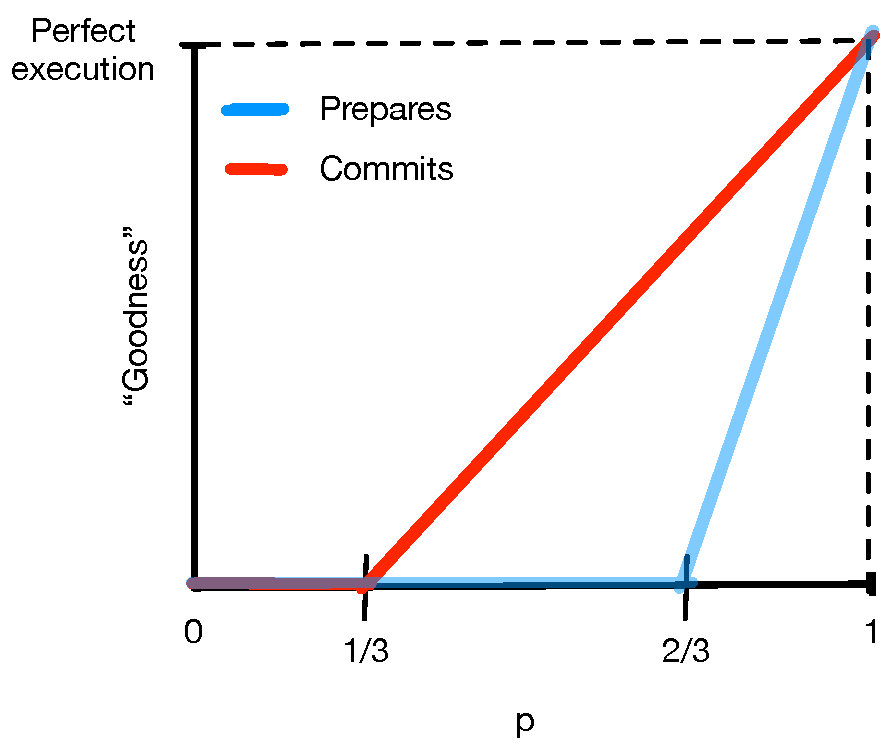
\includegraphics[width=3in]{goodness-with-p.pdf} \label{fig:utility} }
	\subfloat[\NCCP and \NPCP as a function of $\alpha$]{ 	
\includegraphics[width=3in]{cs.pdf} \label{fig:collectivepenalties} }
	
	\caption{Plotting the griefing factor as a function of the proportion of players coordinating to grief.}
	\label{fig:GF}
\end{figure}


In the normal case, anything less than $\frac{1}{3}$ Commits provides no economic security, so we can treat $p_c < \frac{1}{3}$ Commits as equivalent to no Commits; this thus suggests $\NPP = 2 * \NCP$. We can also normalize $\NCP = 1$.

Now, let us analyze the griefing factors, to try to determine an optimal shape for $\NCCP$. The griefing factor for non-Committing is,

\begin{equation}
\mathscr{GF} = \frac{(1-\alpha) * \NCCP(\alpha)}{\alpha * (1 + \NCCP(\alpha))} \; .
\end{equation}

The griefing factor for censoring is the inverse of this. If we want the griefing factor for non-Committing to equal one, then we could compute:

\begin{eqnarray}
\alpha * (1 + \NCCP(\alpha)) &=& (1-\alpha) * \NCCP(\alpha) \\
\frac{1 + \NCCP(\alpha)}{\NCCP(\alpha)} &=& \frac{1-\alpha}{\alpha} \\
\frac{1}{\NCCP(\alpha)} &=& \frac{1-\alpha}{\alpha} - 1 \\
\NCCP(\alpha) &=& \frac{\alpha}{1-2\alpha}
\end{eqnarray}

Note that for $\alpha = \frac{1}{2}$, this would set the \NCCP to infinity. Hence, with this design a griefing factor of $1$ is infeasible. We \emph{can} achieve that effect in a different way - by making \NCP itself a function of $\alpha$; in this case, $\NCCP = 1$ and $\NCP = \max[0, 1 - 2\alpha]$ would achieve the desired effect. If we want to keep the formula for \NCP constant, and the formula for \NCCP reasonably simple and bounded, then one alternative is to set $\NCCP(\alpha) = \frac{\alpha}{1-\alpha}$; this keeps griefing factors bounded between $\frac{1}{2}$ and $2$.

\section{Pools}

In a traditional (i.e., not sharded or otherwise scalable) blockchain, there is a limit to the number of validators that can be supported, because each validator imposes a substantial amount of overhead on the system. If we accept a maximum overhead of two consensus messages per second, and an epoch time of 1400 seconds, then this means that the system can handle 1400 validators (not 2800 because we need to count prepares and commits). Given that the number of individual users interested in staking will likely exceed 1400, this necessarily means that most users will participate through some kind of ``stake pool''.

There are several possible kinds of stake pools:

\begin{itemize}
\item \textbf{Fully centrally managed}: users $B_1 \ldots B_n$ send coins to pool operator $A$. $A$ makes a few deposit transactions containing their combined balances, fully controls the Prepare and Commit process, and occasionally withdraws one of their deposits to accommodate users wishing to withdraw their balances. Requires complete trust.
\item \textbf{Centrally managed but trust-reduced}: users $B_1 \ldots B_n$ send coins to a pool contract. The contract sends a few deposit transactions containing their combined balances, assigning pool operator $A$ control over the Prepare and Commit process, and the task of keeping track of withdrawal requests. $A$ occasionally withdraws one of their deposits to accommodate users wishing to withdraw their balances; the withdrawals go directly into the contract, which ensures each user's right to withdraw a proportional share. Users need to trust the operator not to get their deposits penalized, but the operator cannot steal the coins. The trust requirement can be reduced further if the pool operator themselves contributes a large portion of the coins, as this will disincentivize them from staking maliciously.
\item \textbf{2-of-3}: a user makes a deposit transaction and specifies as validation code a 2-of-3 multisig, consisting of (i) the user's online key, (ii) the pool operator's online key, and (iii) the user's offline backup key. The need for two keys to sign off on a prepare, Commit or withdraw minimizes key theft risk, and a liveness failure on the pool side can be handled by the user using their backup key.
\item \textbf{Multisig managed}: users $B_1 \ldots B_n$ send coins to a pool contract that works in the exact same way as a centrally managed pool, except that a multisig of several semi-trusted parties needs to approve each Prepare and Commit message.
\item \textbf{Collective}: users $B_1 \ldots B_n$ send coins to a pool contract that that works in the exact same way as a centrally managed poolg
, except that a threshold signature of at least portion $p$ of the users themselves (say, $p = 0.6$) needs to approve each Prepare and Commit messagge.
\end{itemize}

We expect pools of different types to emerge to accomodate smaller users. In the long term, techniques such as blockchain sharding will make it possible to increase the number of users that can validate directly, and extensions to allow validators to temporarily ``drop out'' from the validator set when they are offline can mitigate liveness risk.

\section{Conclusions}

The above analysis gives a parametrized scheme for incentivizing in Casper, and shows that it is a Nash equilibrium in an uncoordinated-choice model with a wide variety of settings. We then attempt to derive one possible set of specific values for the various parameters by starting from desired objectives, and choosing values that best meet the desired objectives. This analysis does not include non-economic attacks, as those are covered by other materials, and does not cover more advanced economic attacks, including extortion and discouragement attacks. We hope to see more research in these areas, as well as in the abstract theory of what considerations should be taken into account when designing reward and penalty schedules.


\textbf{Future Work.} We would like to see a better protocol utility function \eqref{eq:utilityfunction}.  \todo{fill me in}

\textbf{Acknowledgements.}  We thank Virgil Griffith for review.

%\section{References}
\bibliographystyle{abbrv}
\bibliography{ethereum}

\appendix
\clearpage
\part*{Appendix}

\section{Safety Failure}
\label{app:safetyfailure}
\todo{Put the full description/definition of conflicting blocks here.}




\section{Unused text}

\todo{This is where text goes that for which a home hasn't been found yet.  If no home is found, it will be deleted.}

Two other reasons to participate in stake pools are (i) to mitigate \emph{key theft risk} (i.e. an attacker hacking into their online machine and stealing the key), and (ii) to mitigate \emph{liveness risk}, the possibility that the validator node will go offline, perhaps because the operator does not have the time to manage a high-uptime setup.


\todo{Do we want to require that the Prepare be done in the first 1/2 of the epoch?  I'm mildly concerned there may not always be enough time to Commit.}

\todo{Remember: The only block you're allowed to Prepare is the last block of each epoch.}

\todo{Remember: Even if the Finalization goes through, the collective penalties are still applied.}


\textbf{Questions}
\begin{itemize}
\item It's unclear to me why we need $\epochsource$ in the Prepare.

\end{itemize}


\end{document}
        